\section{\texorpdfstring{Comparison with Previous Analyses}{Comparison with Previous Analyses}}
\label{sec:comparewpreviouse}
The comparison between $\pi^0$ double ratio and $\pi^{\pm}$ double ratio is of interest because charged pions and $\pi^0$ contain similar fav and disfav Collins Fragmentation functions as shown in Eqs.~\eqref{eqn:allratiosexpress1}-\eqref{eqn:allratiosexpress3}. Also theorist predict that the UC asymmetry is approximately equal to $\pi^0$ asymmetry~\cite{CollinsInSIDISandEE}. To do the comparison, charged pions to thrust open angle is limited below 0.3, the same with $\pi^0$ open angle constraint. Also $z>0.1$ is applied on charged pion pairs. The double ratios for charged pion is given in Eq.~\eqref{eqn:chargeddoubleratio1},.~\eqref{eqn:chargeddoubleratio2}. 
\begin{equation}
\begin{aligned}
UL&=&\frac{A^U}{A^L}&=&\frac{\pi^+\pi^-}{\pi^+\pi^++\pi^-\pi^-}
\label{eqn:chargeddoubleratio1}
\end{aligned}
\end{equation}

\begin{equation}
\begin{aligned}
UC&=&\frac{A^U}{A^C}&=&\frac{\pi^+\pi^-}{\pi^+\pi^++\pi^-\pi^-+\pi^+\pi^-+\pi^-\pi^+}
\label{eqn:chargeddoubleratio2}
\end{aligned}
\end{equation}


The double ratio related to $\pi^0$ and charged pions can be expressed as\cite{BabarCharged}\cite{ChargedPionResult2}
\begin{equation}
\begin{aligned}
\frac{A^{0\pm}_{12}}{A^L_{12}}&=1+\cos(\phi_1+\phi_2)\frac{\sin^2(\theta)}{1+\cos^2(\theta)} \\
&\times\bigg\{\frac{f((H^{\bot,fav}_1+H^{\bot,dis}_1)(\bar{H}^{\bot,fav}_1+\bar{H}^{\bot,dis}_1))}{(D^{fav}_1+D^{dis}_1)(\bar{D}^{fav}_1+\bar{D}^{dis}_1)}-\frac{f(H^{\bot,fav}_1\bar{H}^{\bot,dis}_1)}{D^{fav}_1\bar{D}^{dis}_1} \bigg\}  
\end{aligned}
\label{eqn:allratiosexpress1}
\end{equation}

\begin{equation}
\begin{aligned}
\frac{A^{U}_{12}}{A^L_{12}}&=1+\cos(\phi_1+\phi_2)\frac{\sin^2(\theta)}{1+\cos^2(\theta)}\\
&\times\bigg\{\frac{f(H^{\bot,fav}_1\bar{H}^{\bot,fav}_1+H^{\bot,dis}_1\bar{H}^{\bot,fav}_1)}{(D^{fav}_1\bar{D}^{fav}_1+D^{dis}_1\bar{D}^{dis}_1)}-\frac{f(H^{\bot,fav}_1\bar{H}^{\bot,dis}_1)}{D^{fav}_1\bar{D}^{dis}_1} \bigg\} 
\end{aligned}
\label{eqn:allratiosexpress2}
\end{equation}
\begin{equation}
\begin{aligned}
\frac{A^{U}_{12}}{A^C_{12}}&=1+\cos(\phi_1+\phi_2)\frac{\sin^2(\theta)}{1+\cos^2(\theta)}\\
&\times\bigg\{\frac{f(H^{\bot,fav}_1\bar{H}^{\bot,fav}_1+H^{\bot,dis}_1\bar{H}^{\bot,fav}_1)}{(D^{fav}_1\bar{D}^{fav}_1+D^{dis}_1\bar{D}^{dis}_1)}\\
&-\frac{f((H^{\bot,fav}_1+H^{\bot,dis}_1)(\bar{H}^{\bot,fav}_1+\bar{H}^{\bot,dis}_1))}{(D^{fav}_1+D^{dis}_1)(\bar{D}^{fav}_1+\bar{D}^{dis}_1)} \bigg\} \\
\end{aligned}
\label{eqn:allratiosexpress3}
\end{equation}
Just like $\pi^0$, the thrust smearing effect should be considered for charged pions. Here the same method has been used as described in section~\ref{sec:pi0thrustcorrection}. The statistics are too low to have a reliable thrust correction factor for some bins, and those numbers are estimated based on the Belle Monte Carlo results. Details about these estimations can be found in section~\ref{sec:appendix}. For a simple comparison only thrust correction has been considered for charged pions.
\iffalse
\begin{figure}[H]
  \centering     
  \subfigure[$z_1$ bins]{\label{fig:sinzCN}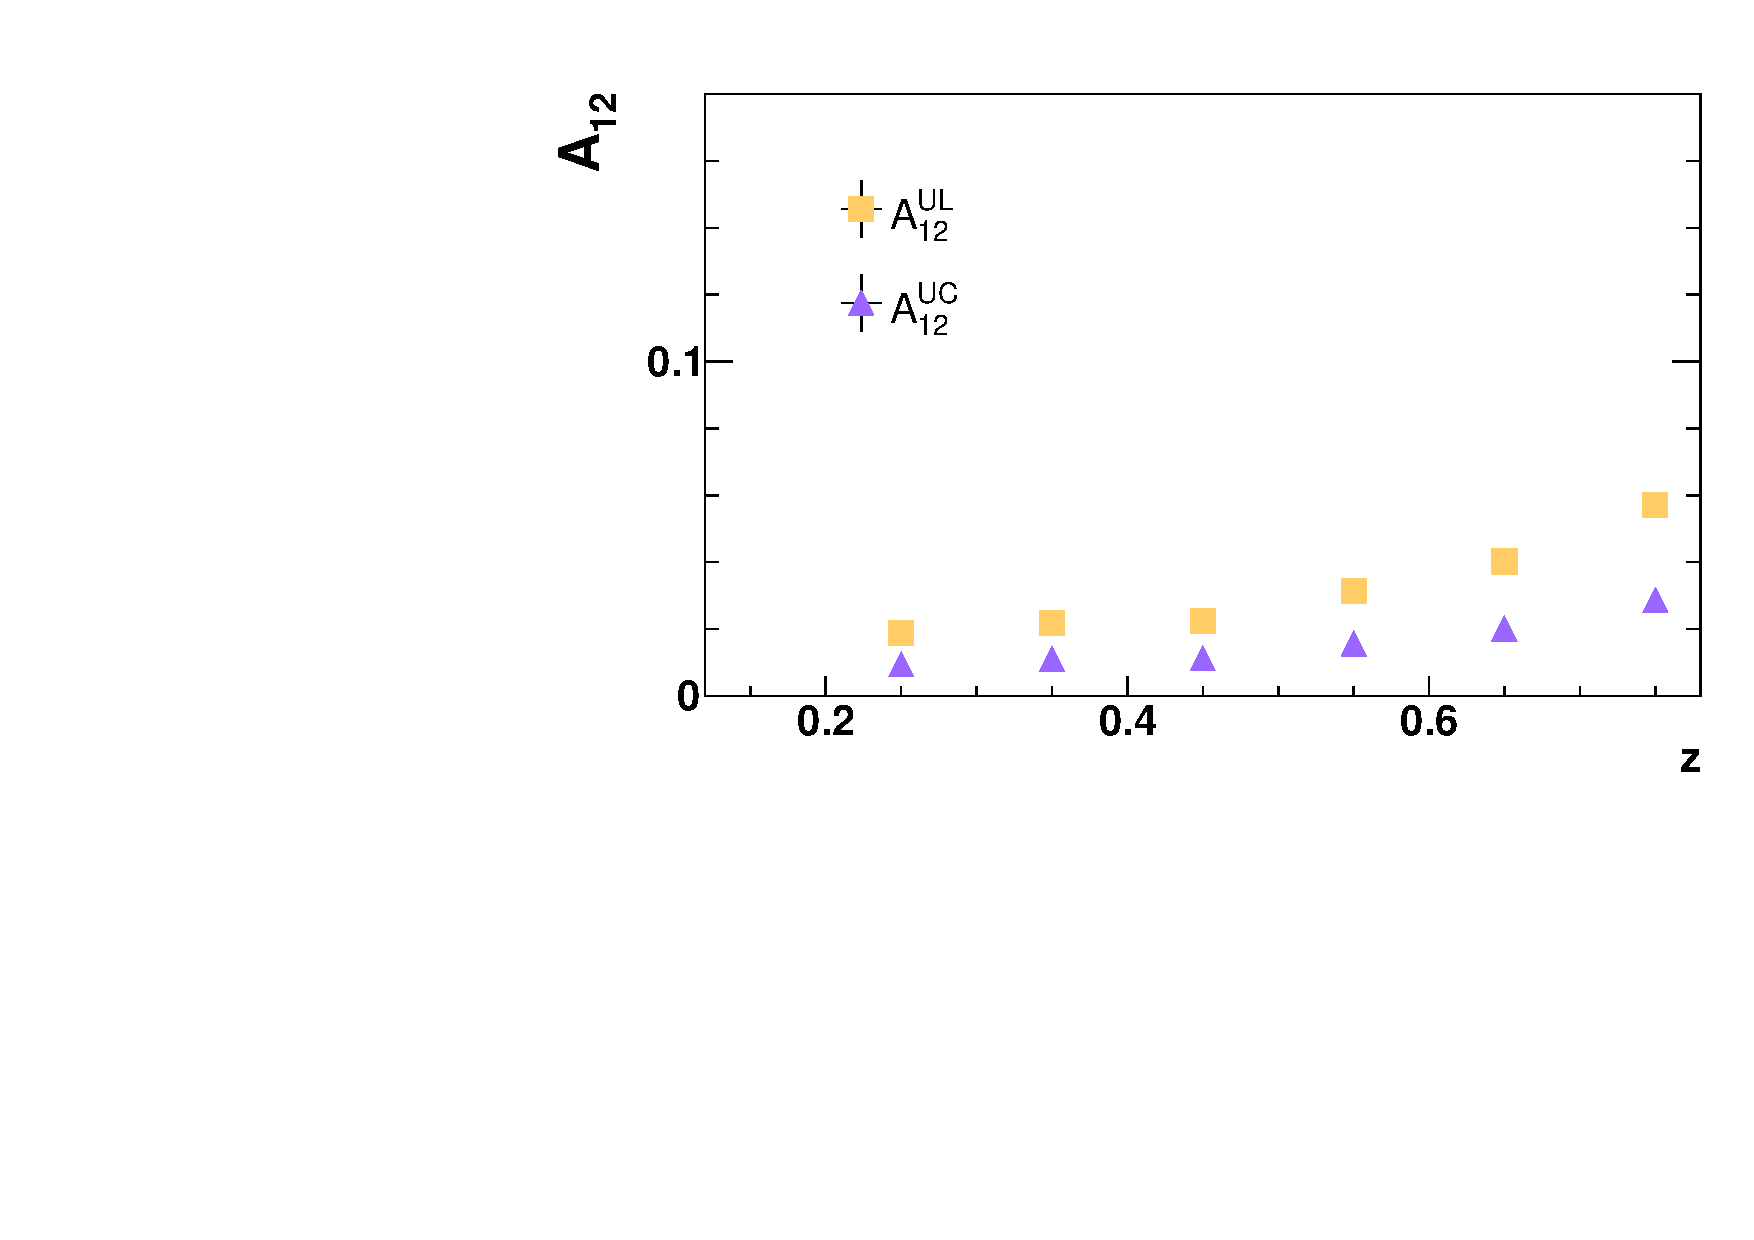
\includegraphics[width=60mm,natwidth=600,natheight=400]{figure_asy/Charged0.pdf}}
  \subfigure[$P_{t1}$ bins]{\label{fig:sinptCN}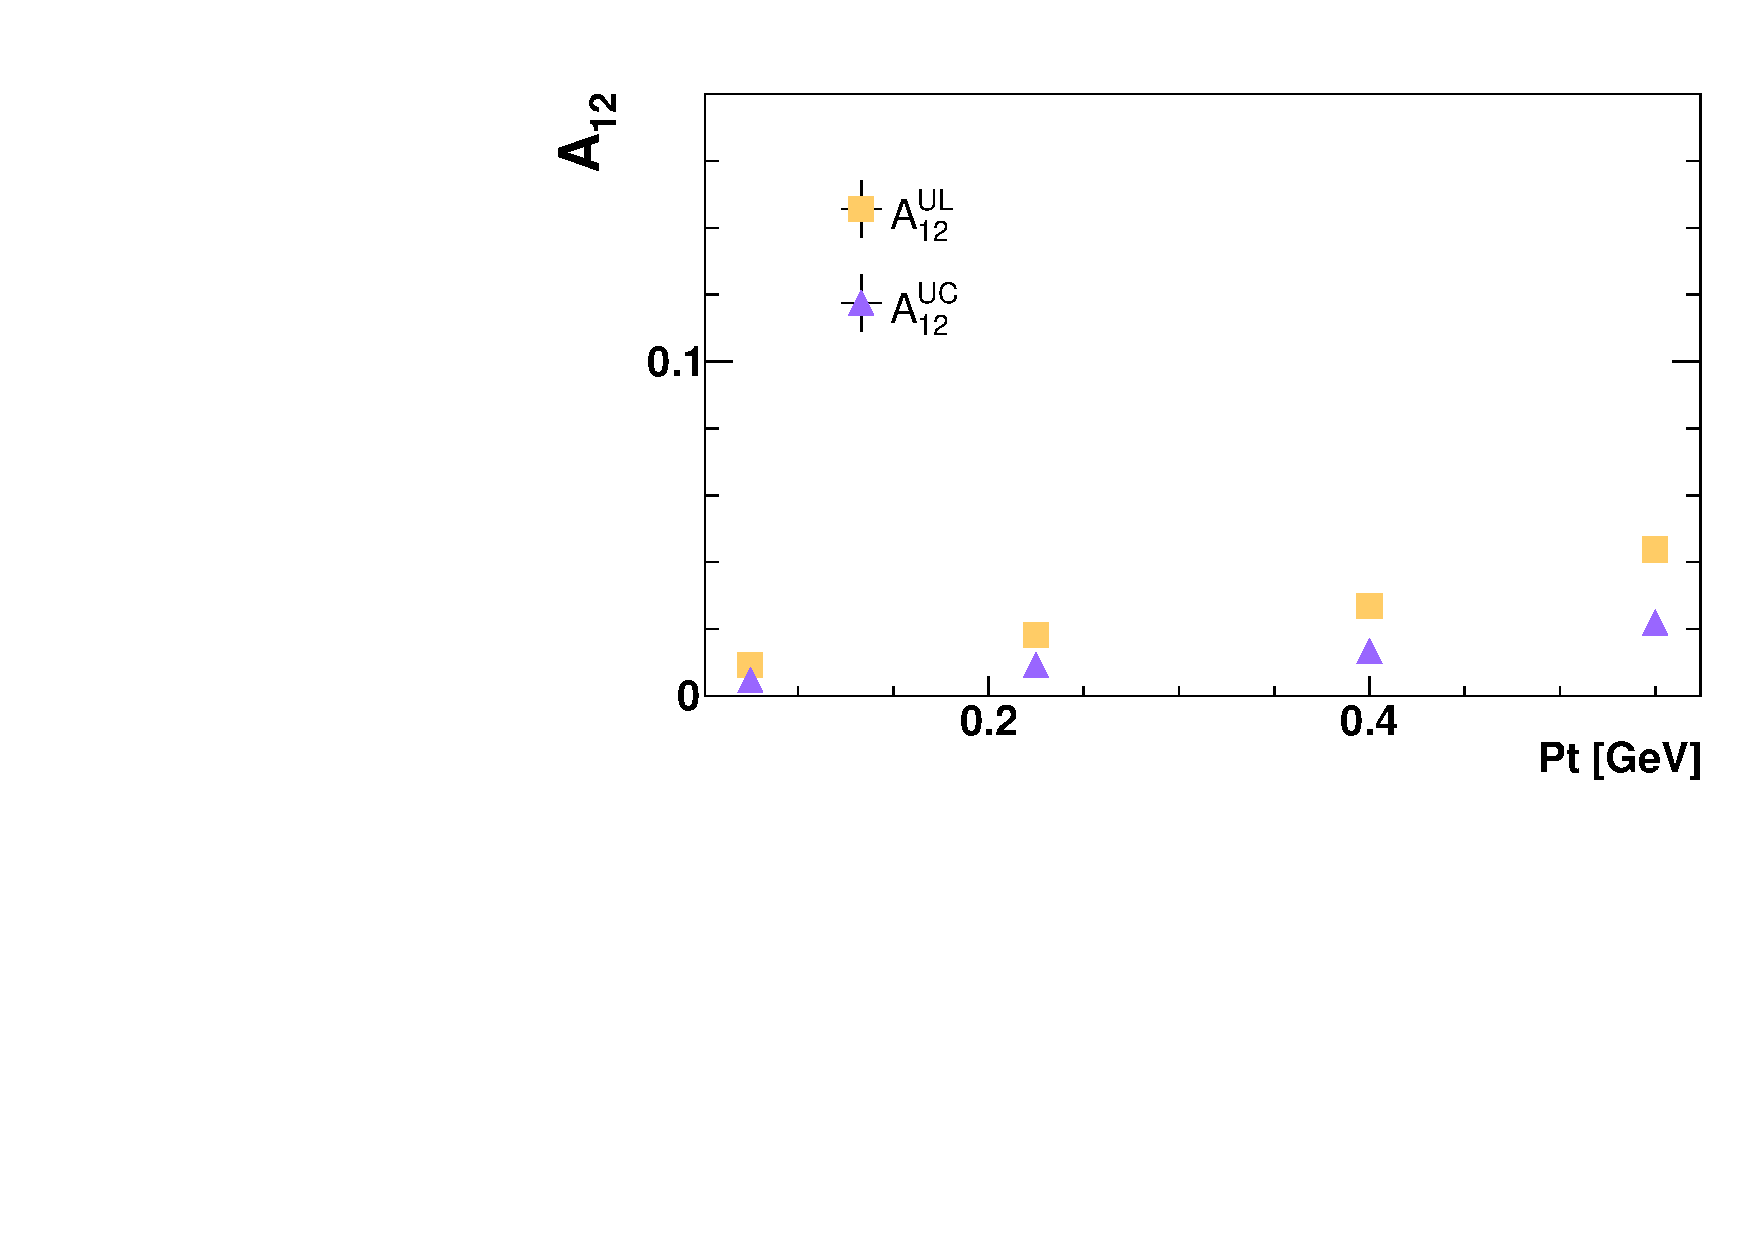
\includegraphics[width=60mm,natwidth=600,natheight=400]{figure_asy/Charged2.pdf}}
  \subfigure[$(z_1,z_2)$ bins]{\label{fig:comzCN}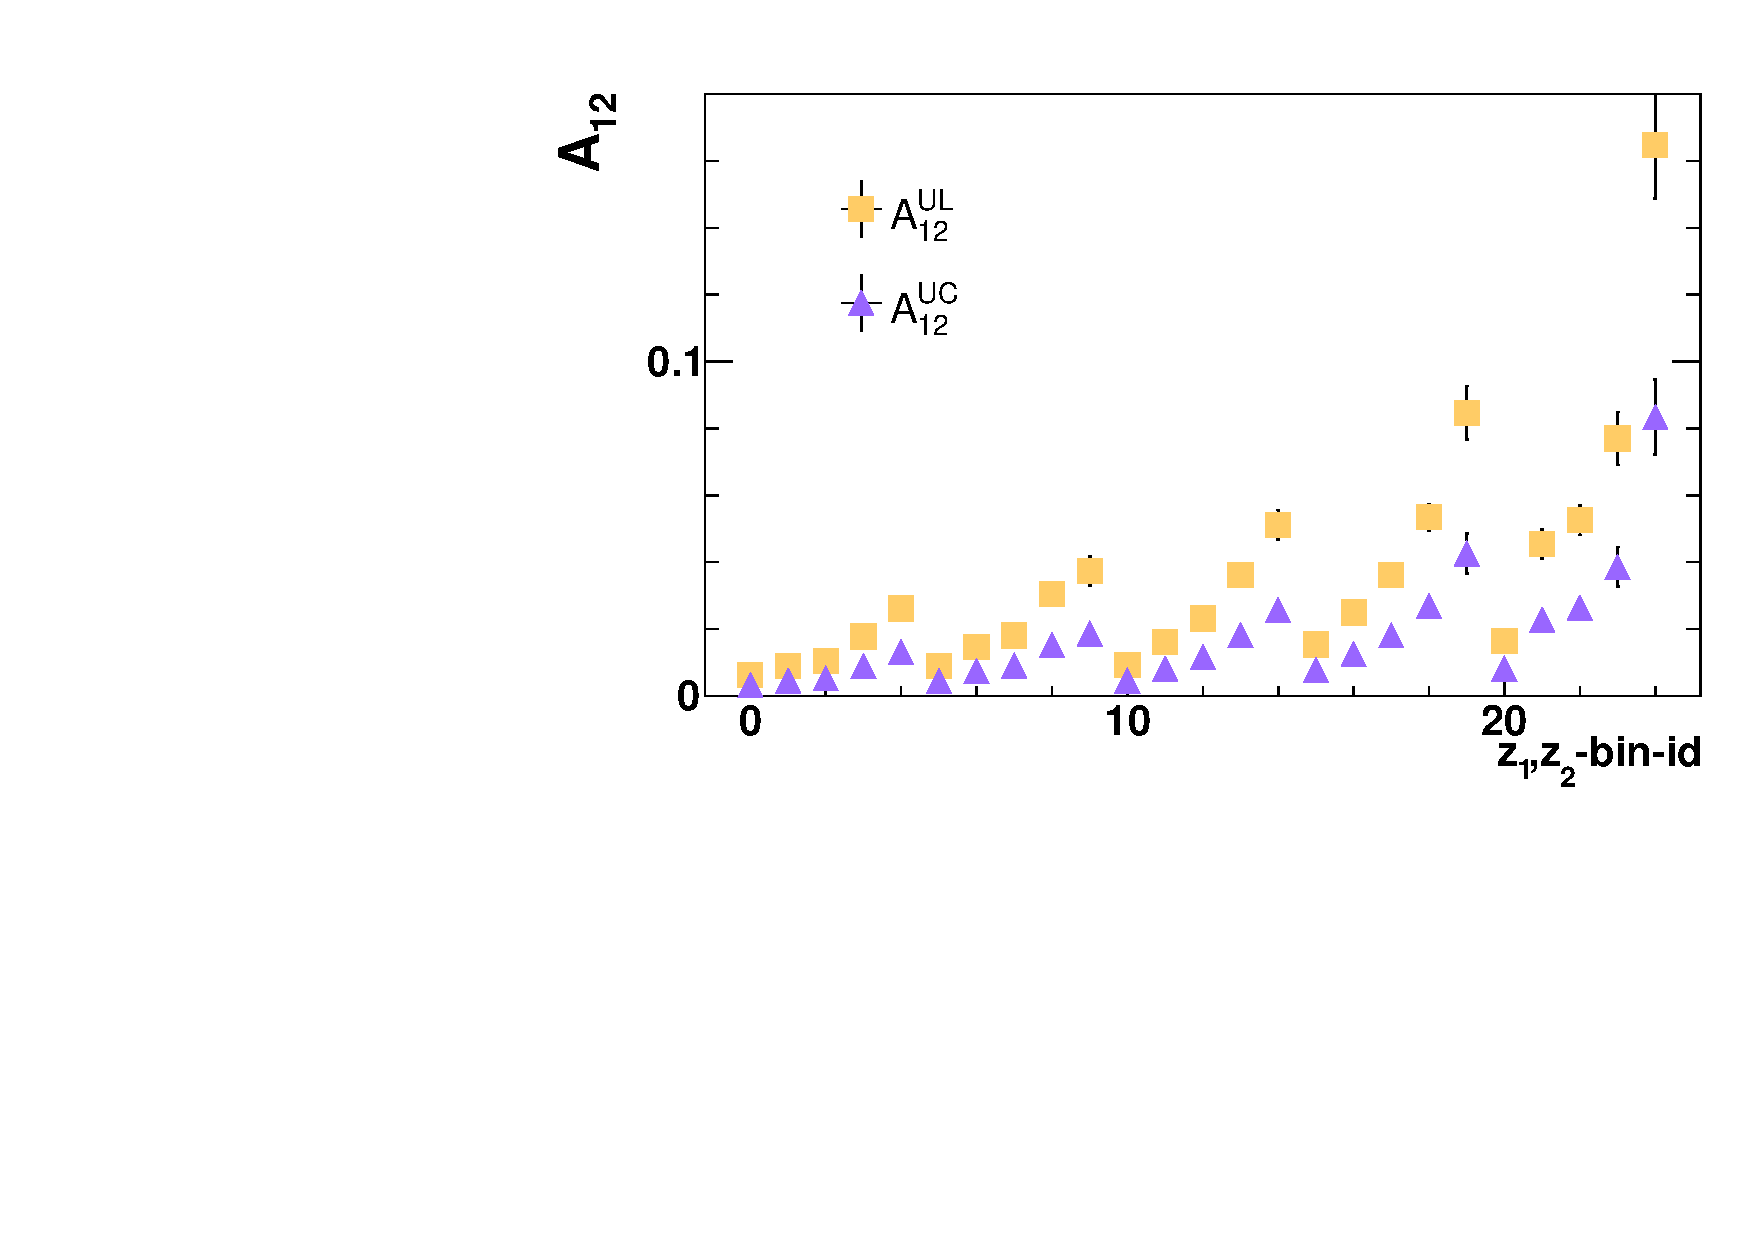
\includegraphics[width=60mm,natwidth=600,natheight=400]{figure_asy/Charged1.pdf}}
  \subfigure[$(P_{t1},P_{t2})$ bins]{\label{fig:comptCN}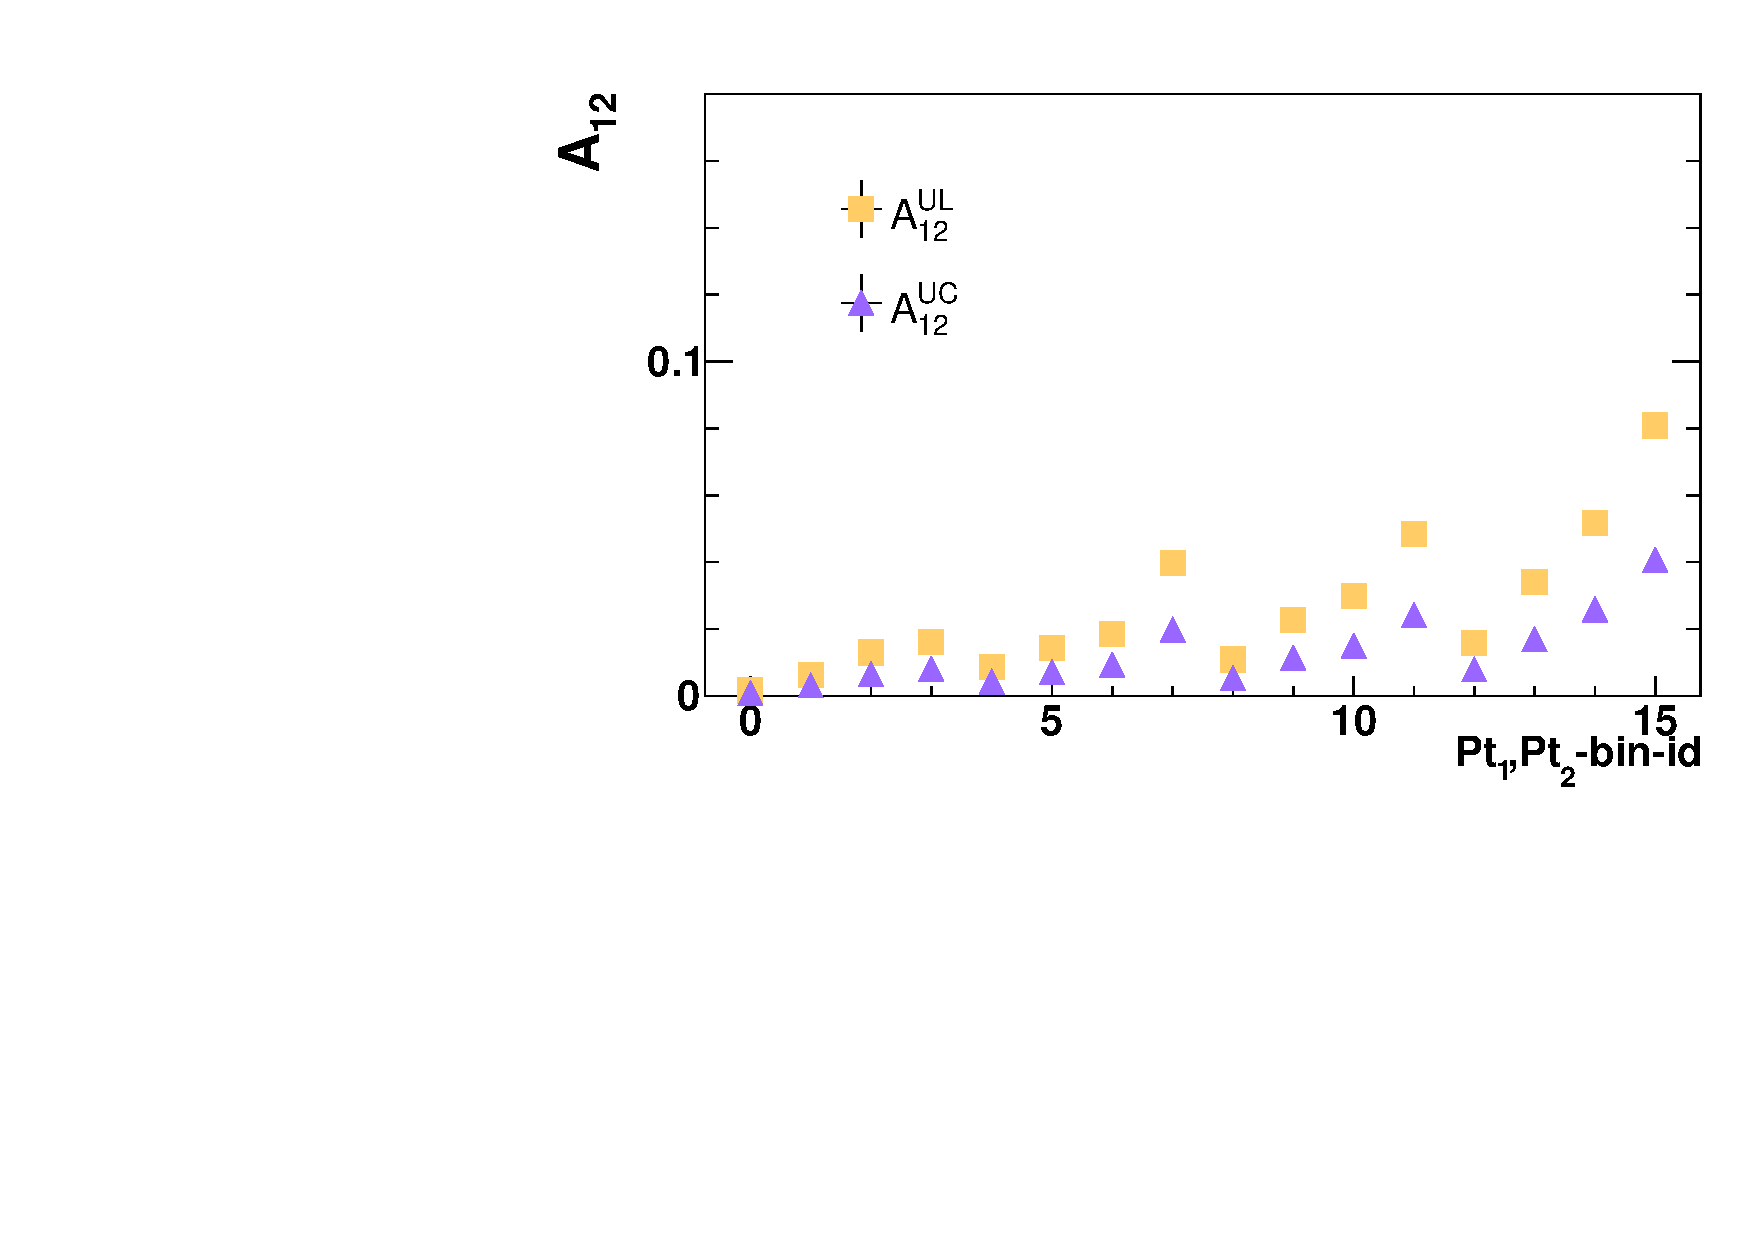
\includegraphics[width=60mm,natwidth=600,natheight=400]{figure_asy/Charged3.pdf}}
  \caption{Charged pion double ratios result for different kinematic bins. The green squares represent no correction result while the purple points are results with thrust smearing correction.}
\label{fig:chargedpion}
\end{figure}
\fi
Fig.~\ref{fig:pionCN} displays the comparison of UL, UC and $\pi^0$ double ratio. In the figure it can be seen that $\pi^0$ double ratio asymmetry is lower than UL double ratio, but it's close to the UC ratios which is consistent with the theorists' prediction. After correcting for the thrust smearing effect, in Fig.~\ref{fig:pionCNcorrection}, the last $(z_1,z_2)$ bins result for charged pion is around 0.25 with large error bar. 
\begin{figure}[H]
  \centering     
  \subfigure[$z_1$ bins]{\label{fig:sinzCN1}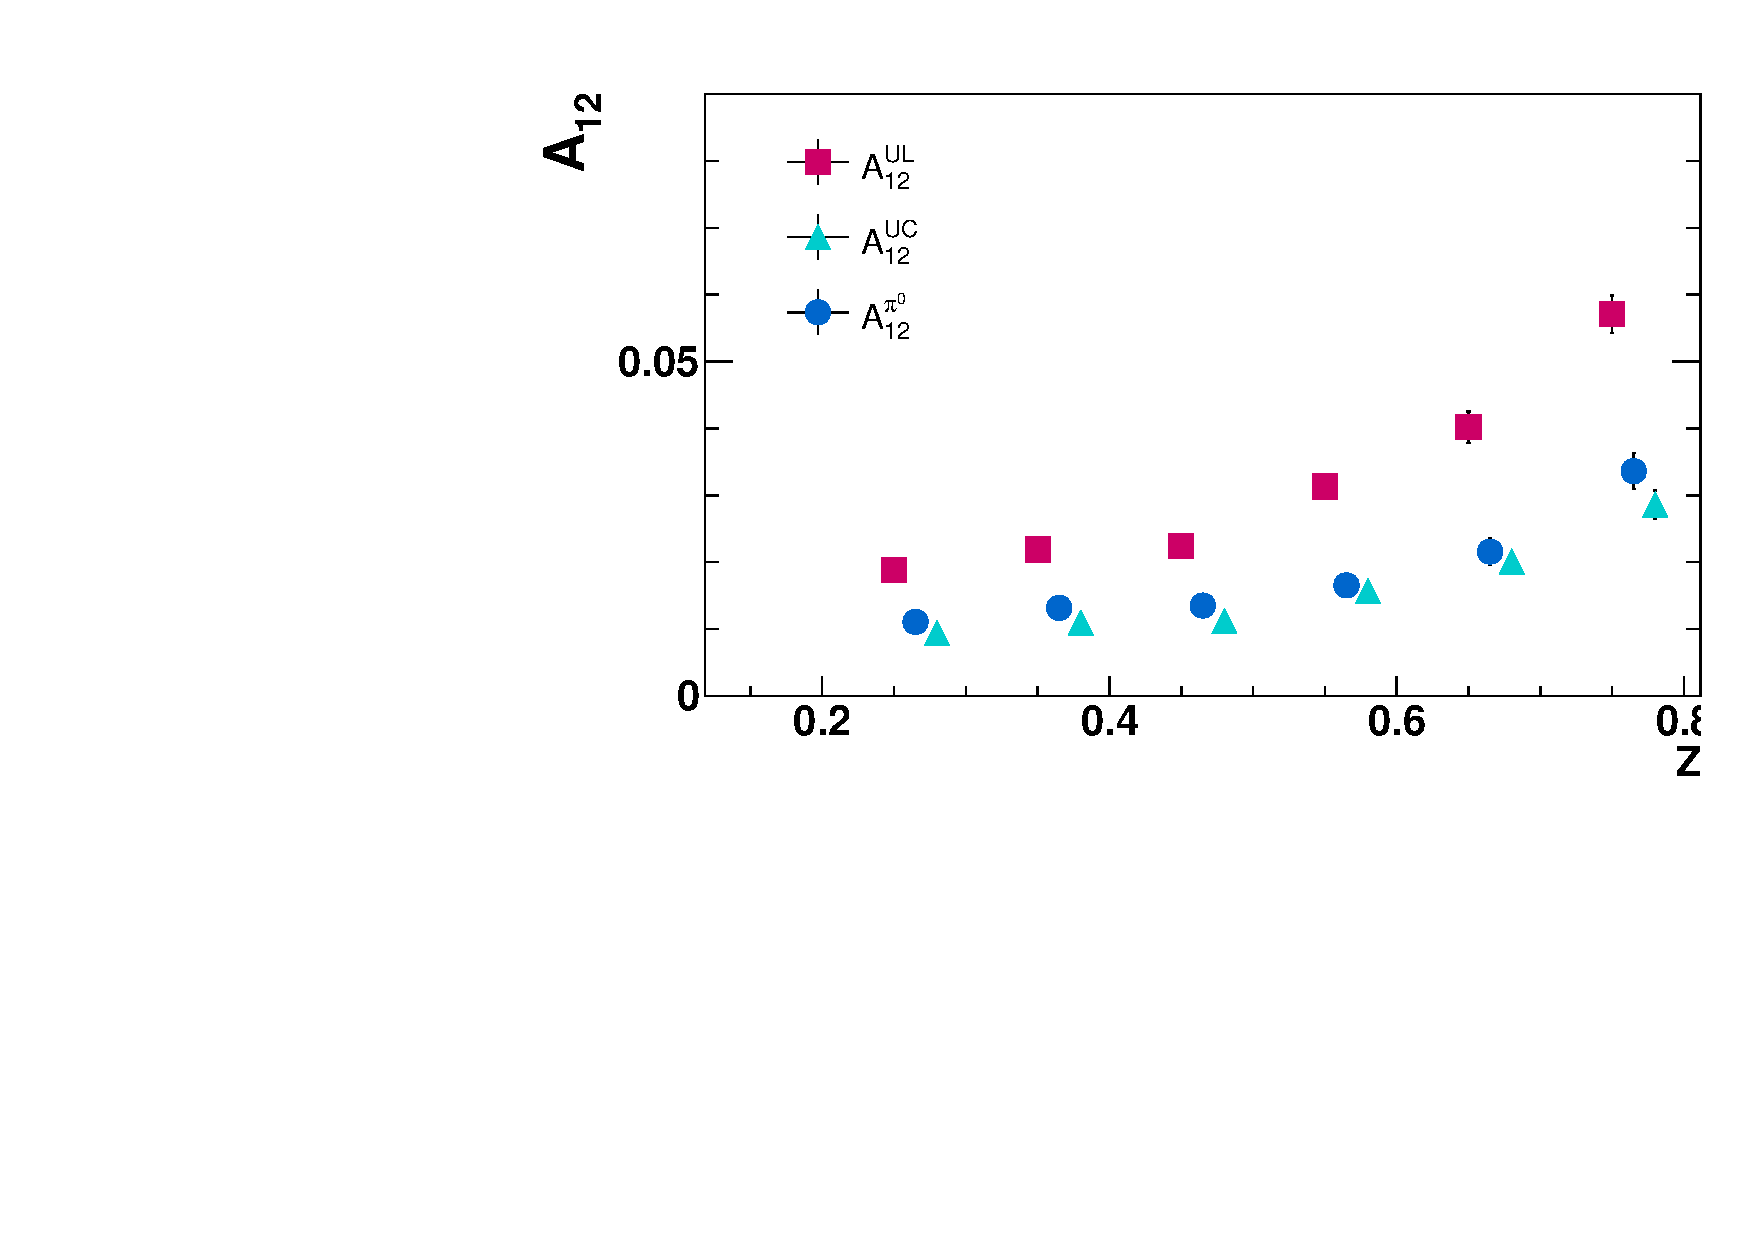
\includegraphics[width=60mm,natwidth=600,natheight=400]{figure_asy/NeutralVsCharge0.pdf}}
  \subfigure[$P_{t1}$ bins]{\label{fig:sinptCN1}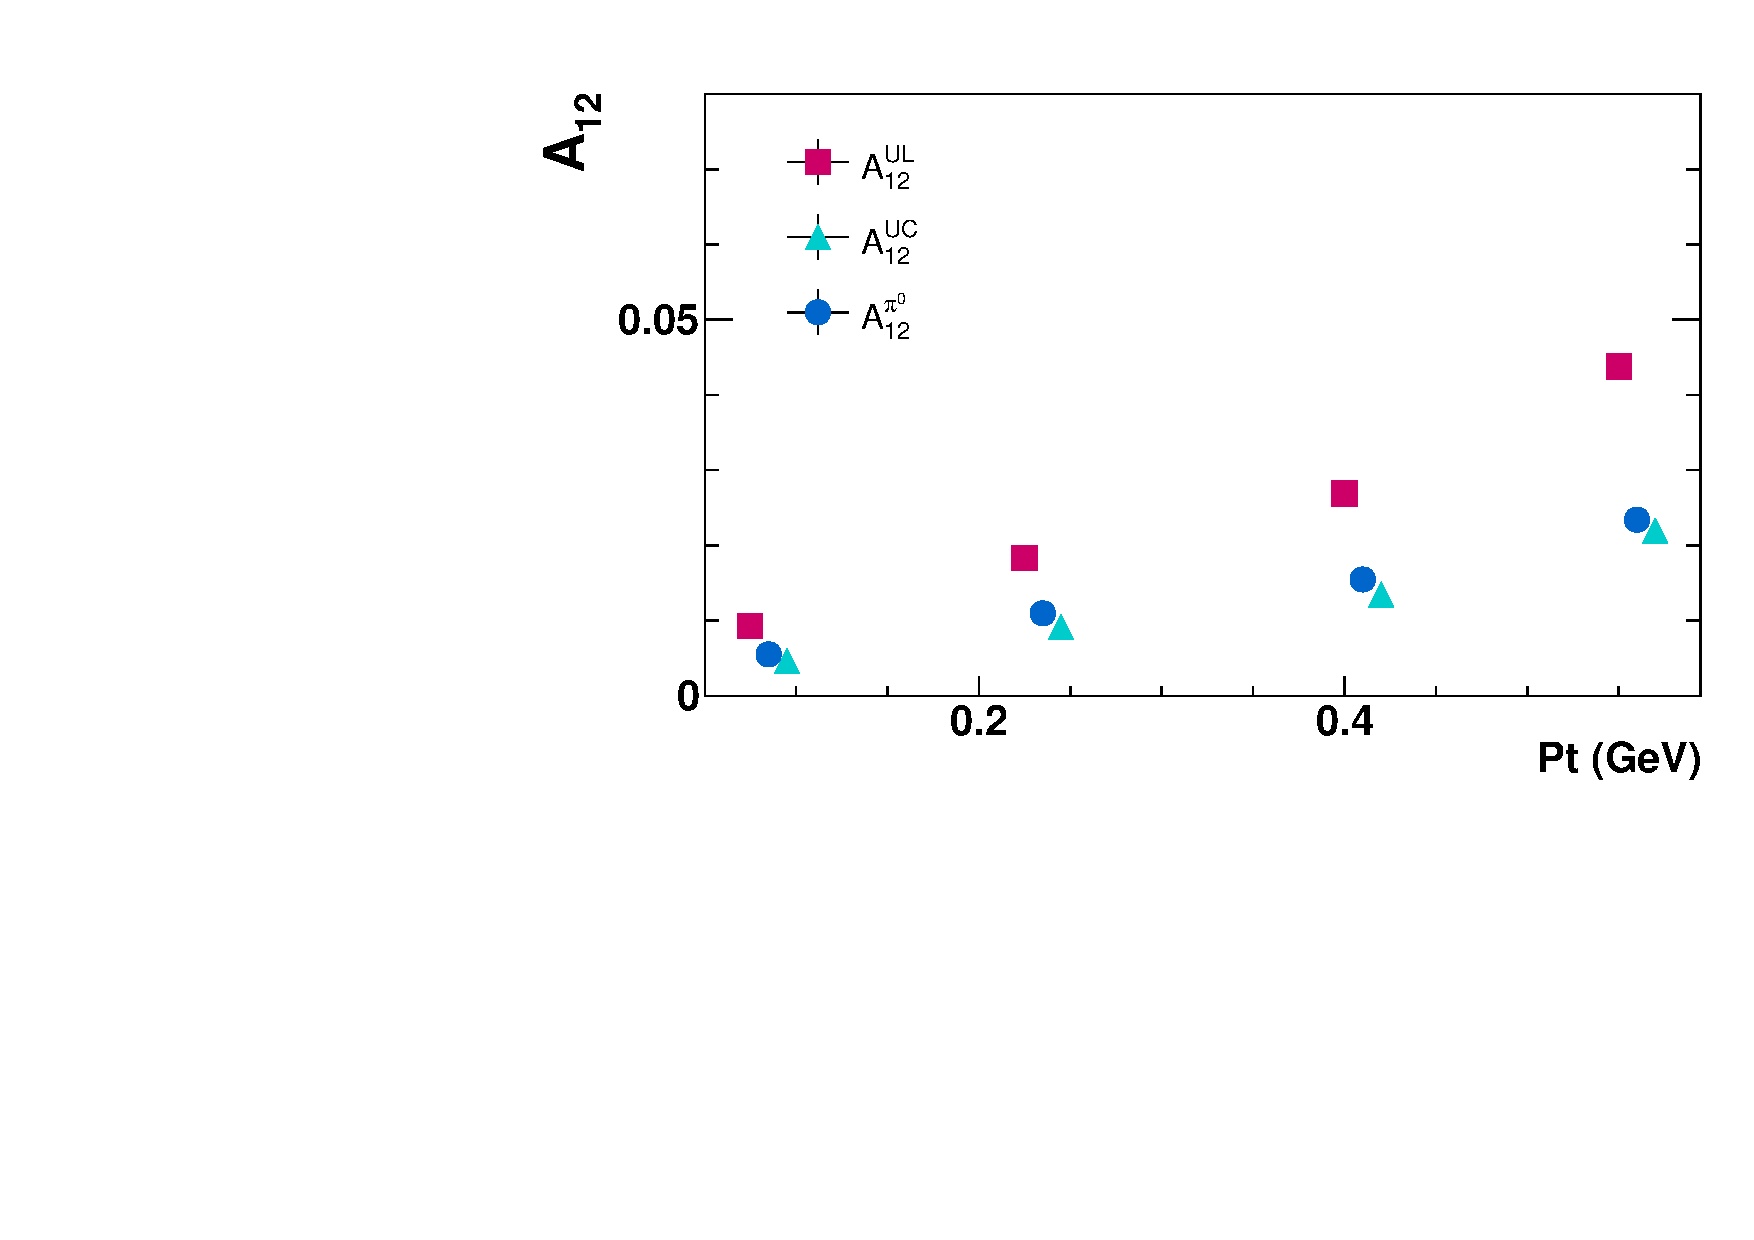
\includegraphics[width=60mm,natwidth=600,natheight=400]{figure_asy/NeutralVsCharge2.pdf}}
  \subfigure[$(z_1,z_2)$ bins]{\label{fig:comzCN1}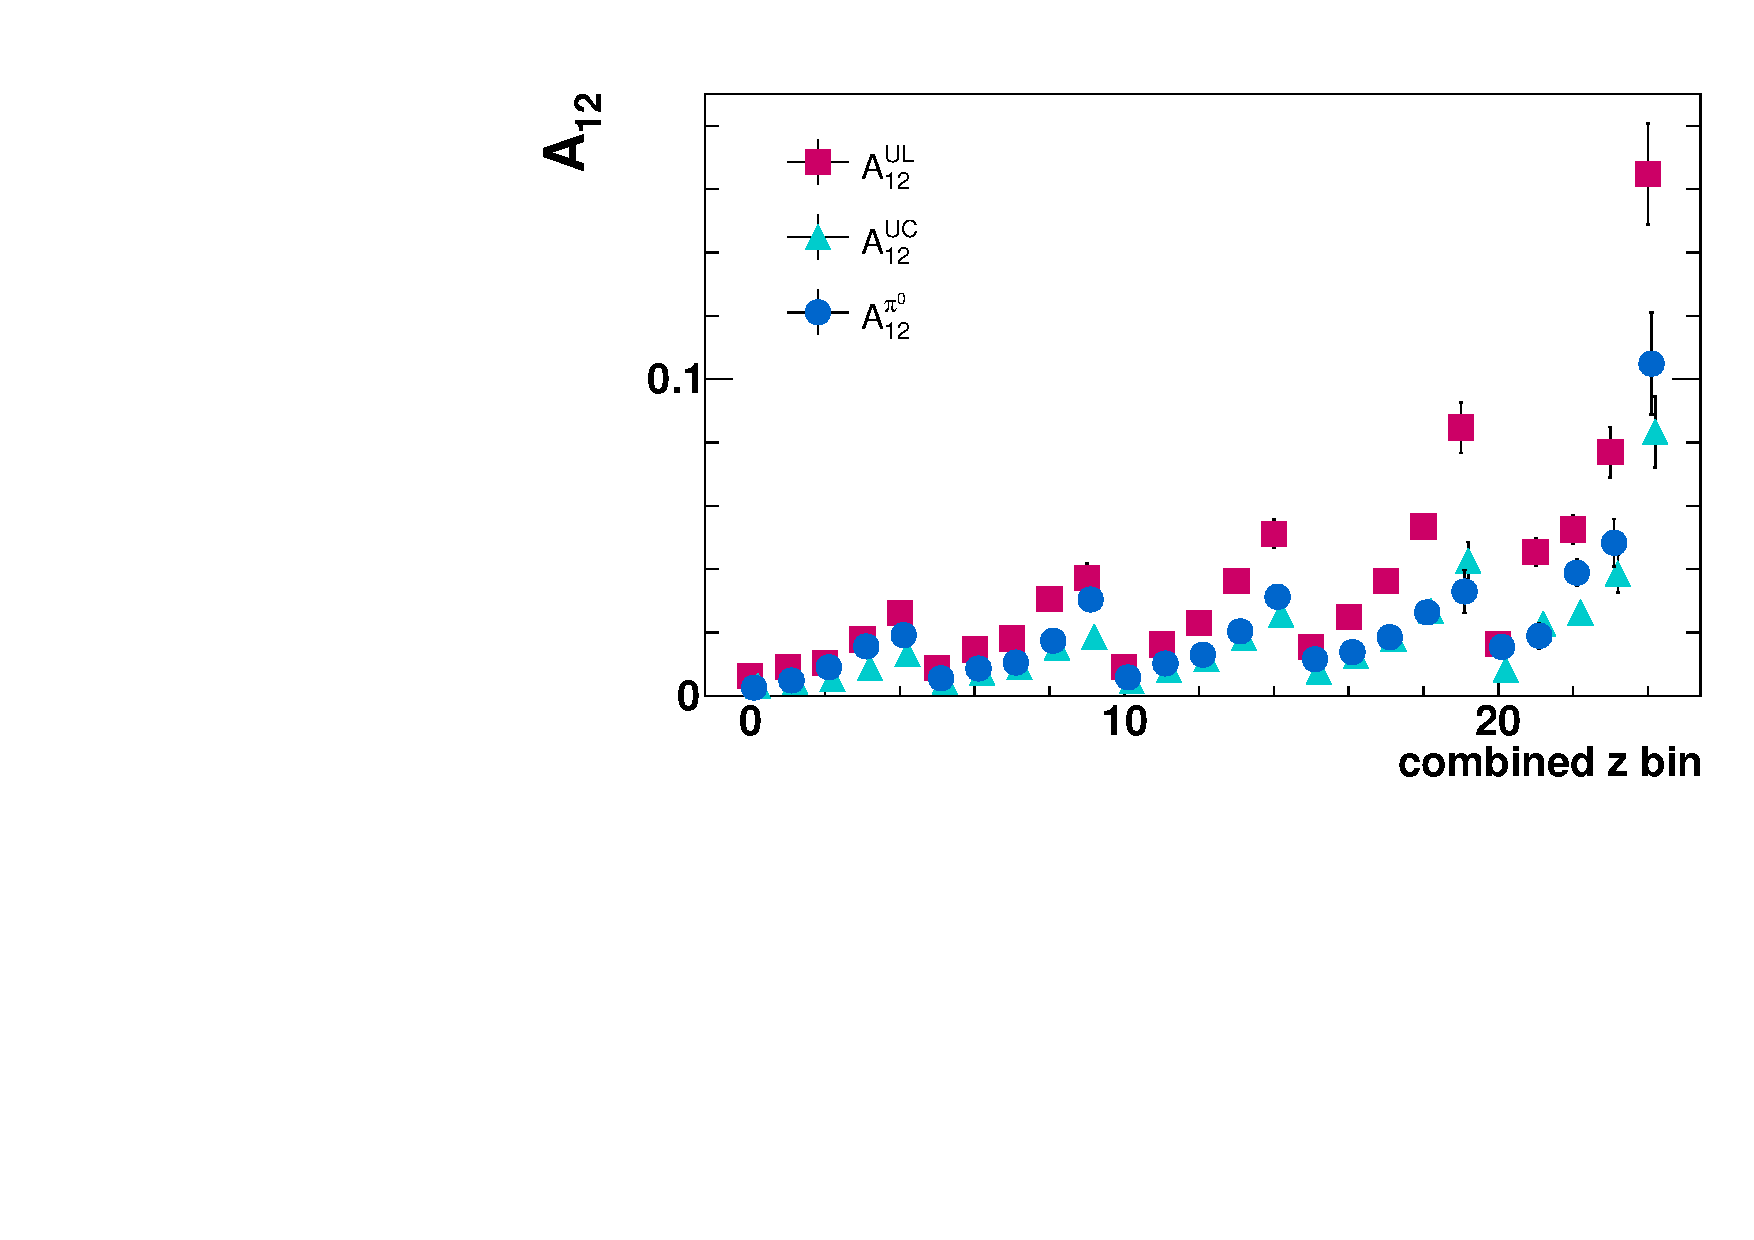
\includegraphics[width=60mm,natwidth=600,natheight=400]{figure_asy/NeutralVsCharge1.pdf}}
  \subfigure[$(P_{t1},P_{t2})$ bins]{\label{fig:comptCN1}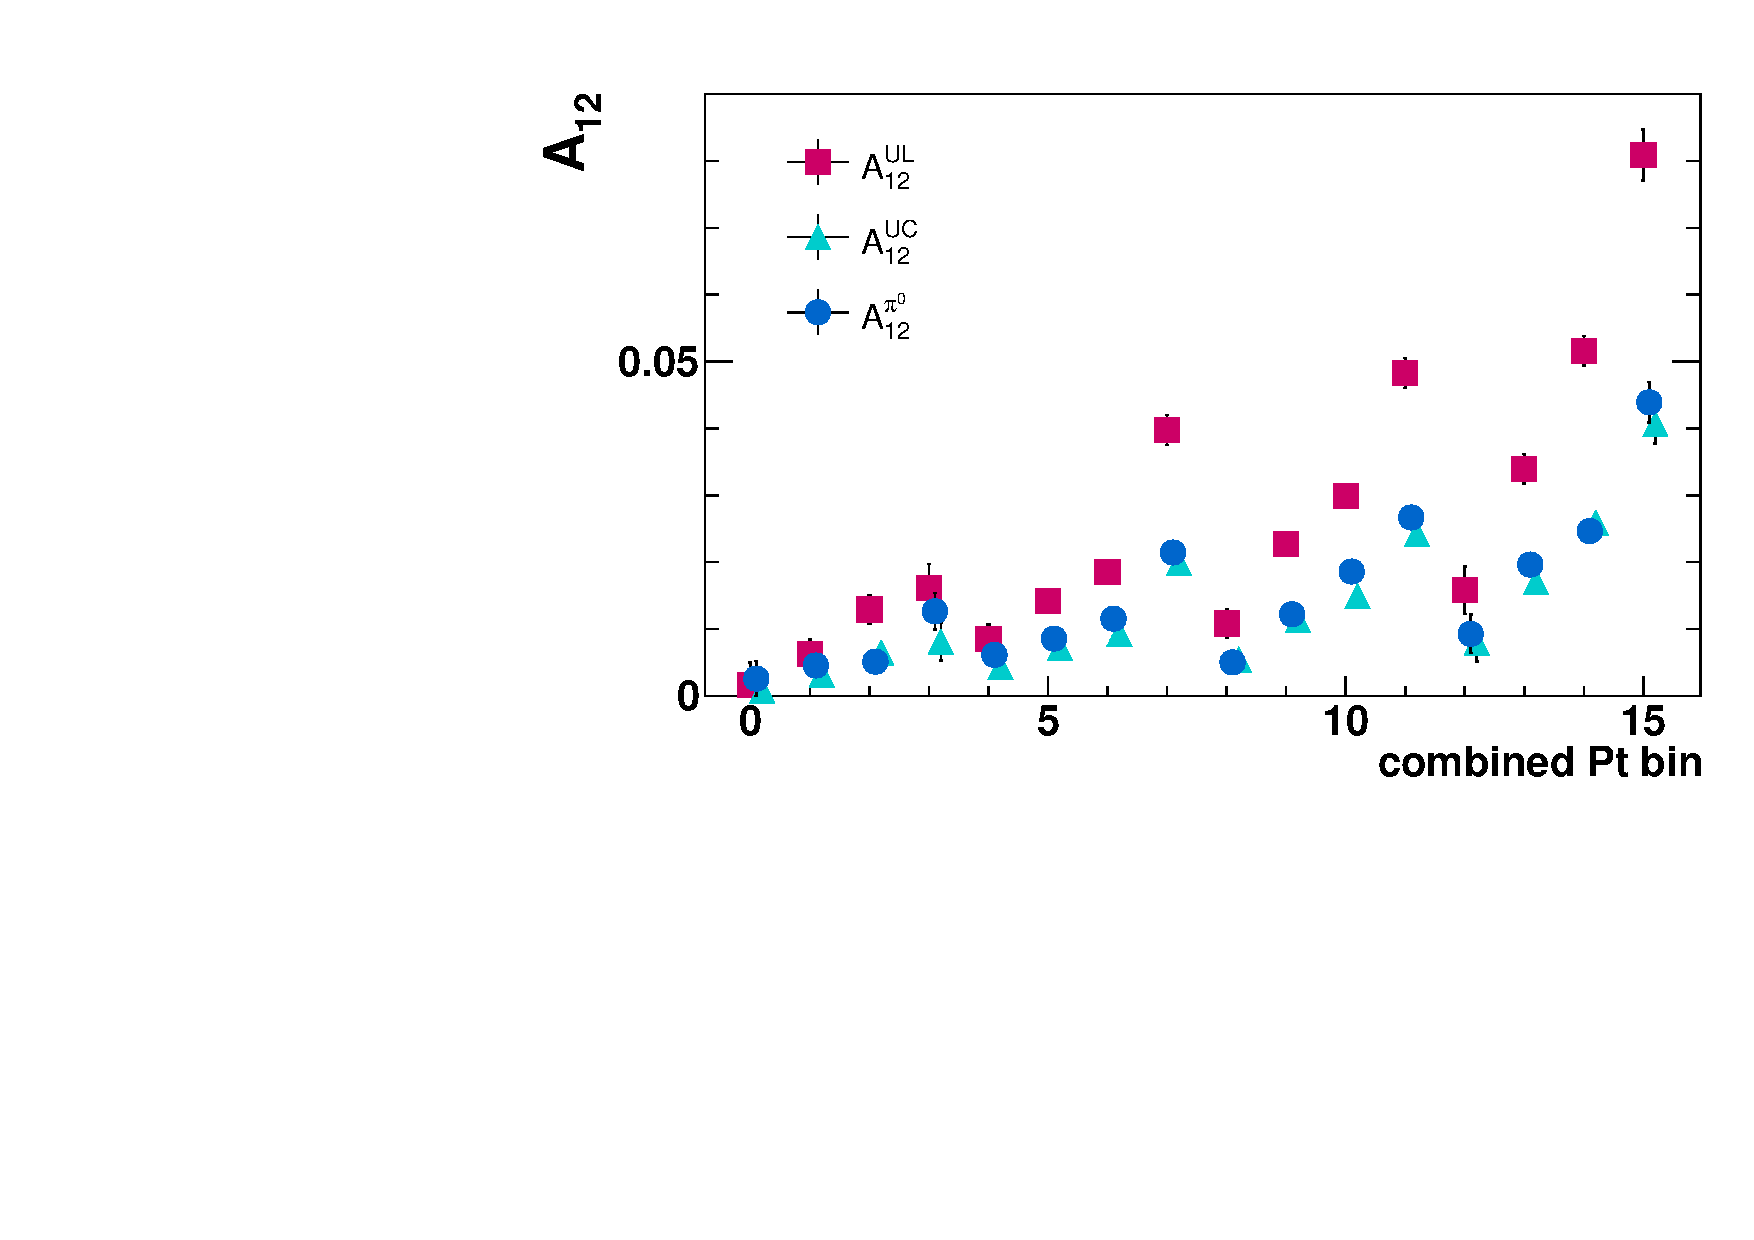
\includegraphics[width=60mm,natwidth=600,natheight=400]{figure_asy/NeutralVsCharge3.pdf}}
  \caption{Charged pion double ratio and $\pi^0$ double ratio versus $z$ or $P_t$. $\pi^0$ double ratio has been modified for background correction. The square, triangle and round points are UL, UC and $\pi^0$ asymmetries, respectively.}
\label{fig:pionCN}
\end{figure}

\begin{figure}[H]
  \centering     
  \subfigure[$z_1$ bins]{\label{fig:sinzCN2}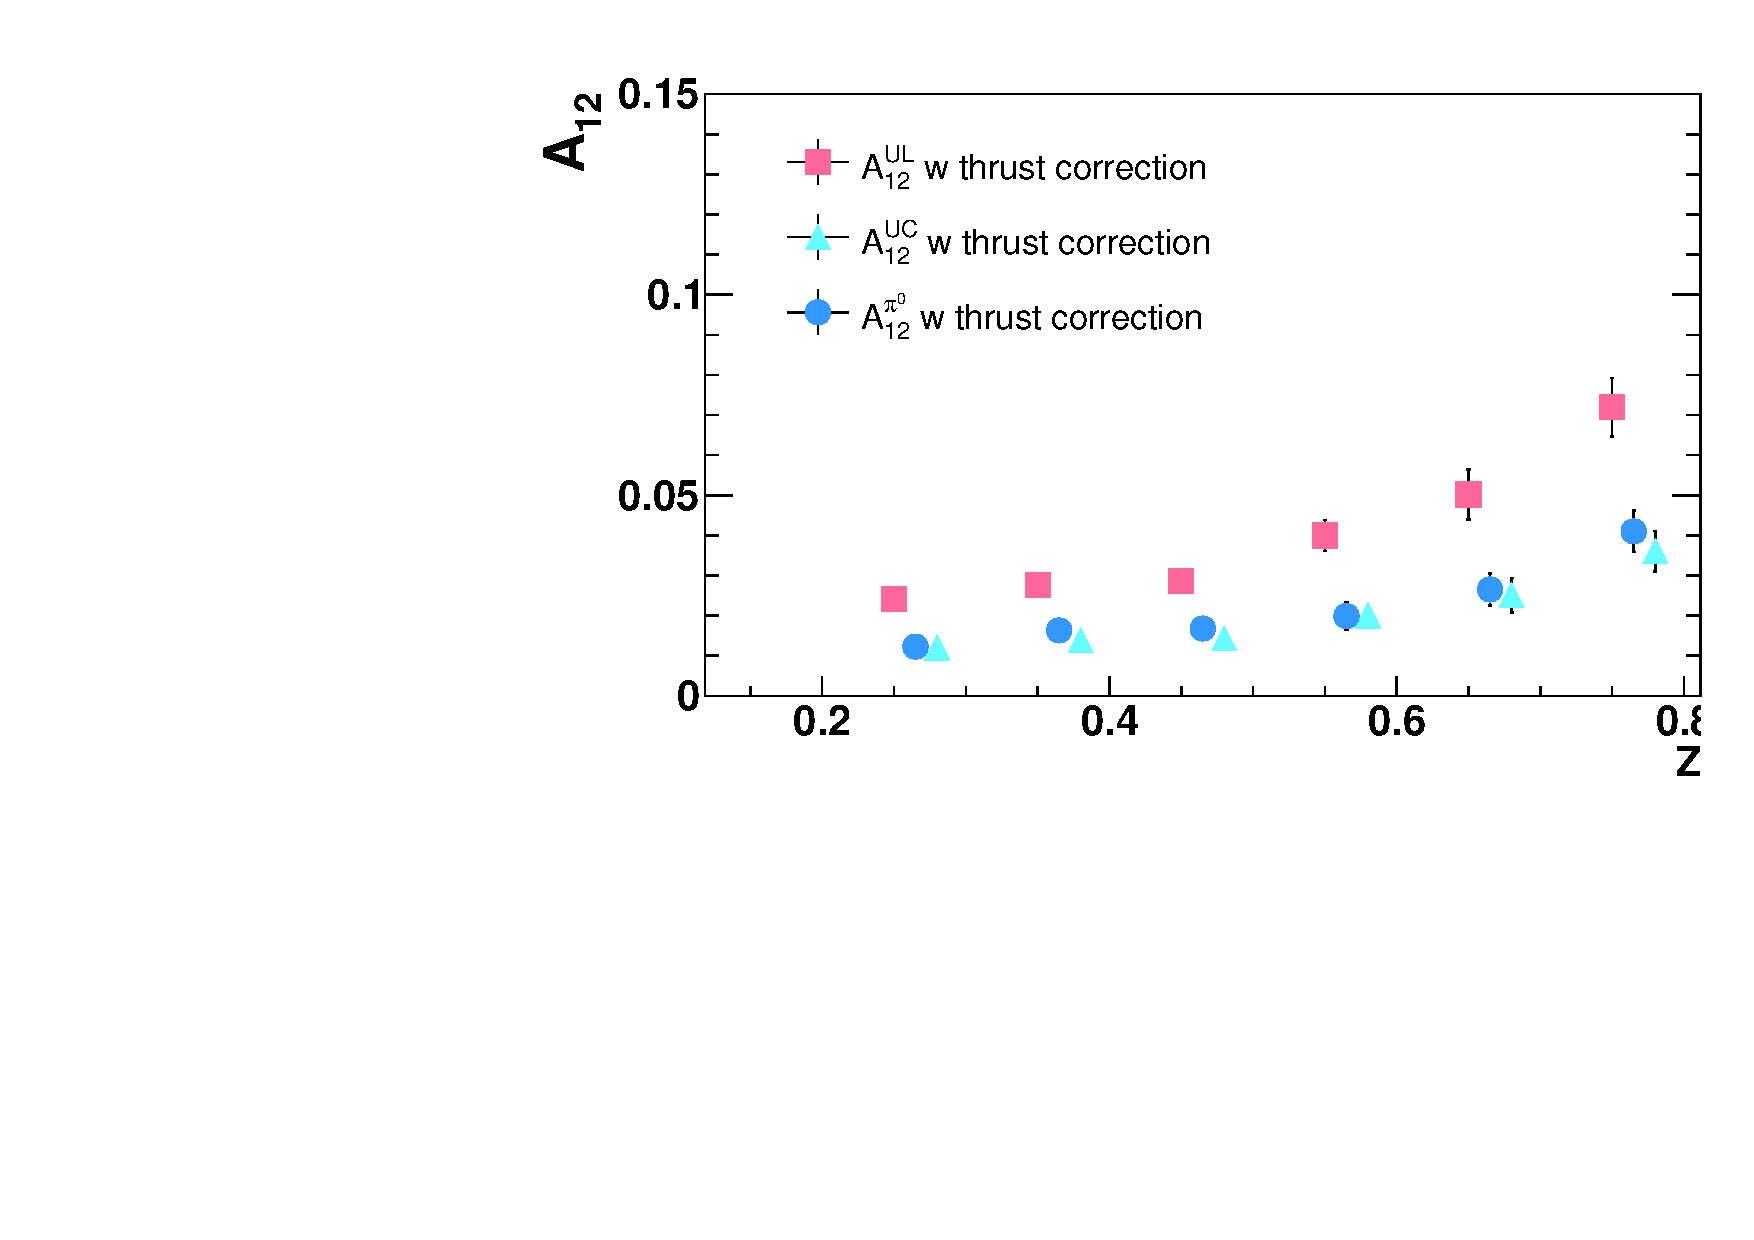
\includegraphics[width=60mm,natwidth=600,natheight=400]{figure_asy/NeutralVsCharge_w_correction0.pdf}}
  \subfigure[$P_{t1}$ bins]{\label{fig:sinptCN2}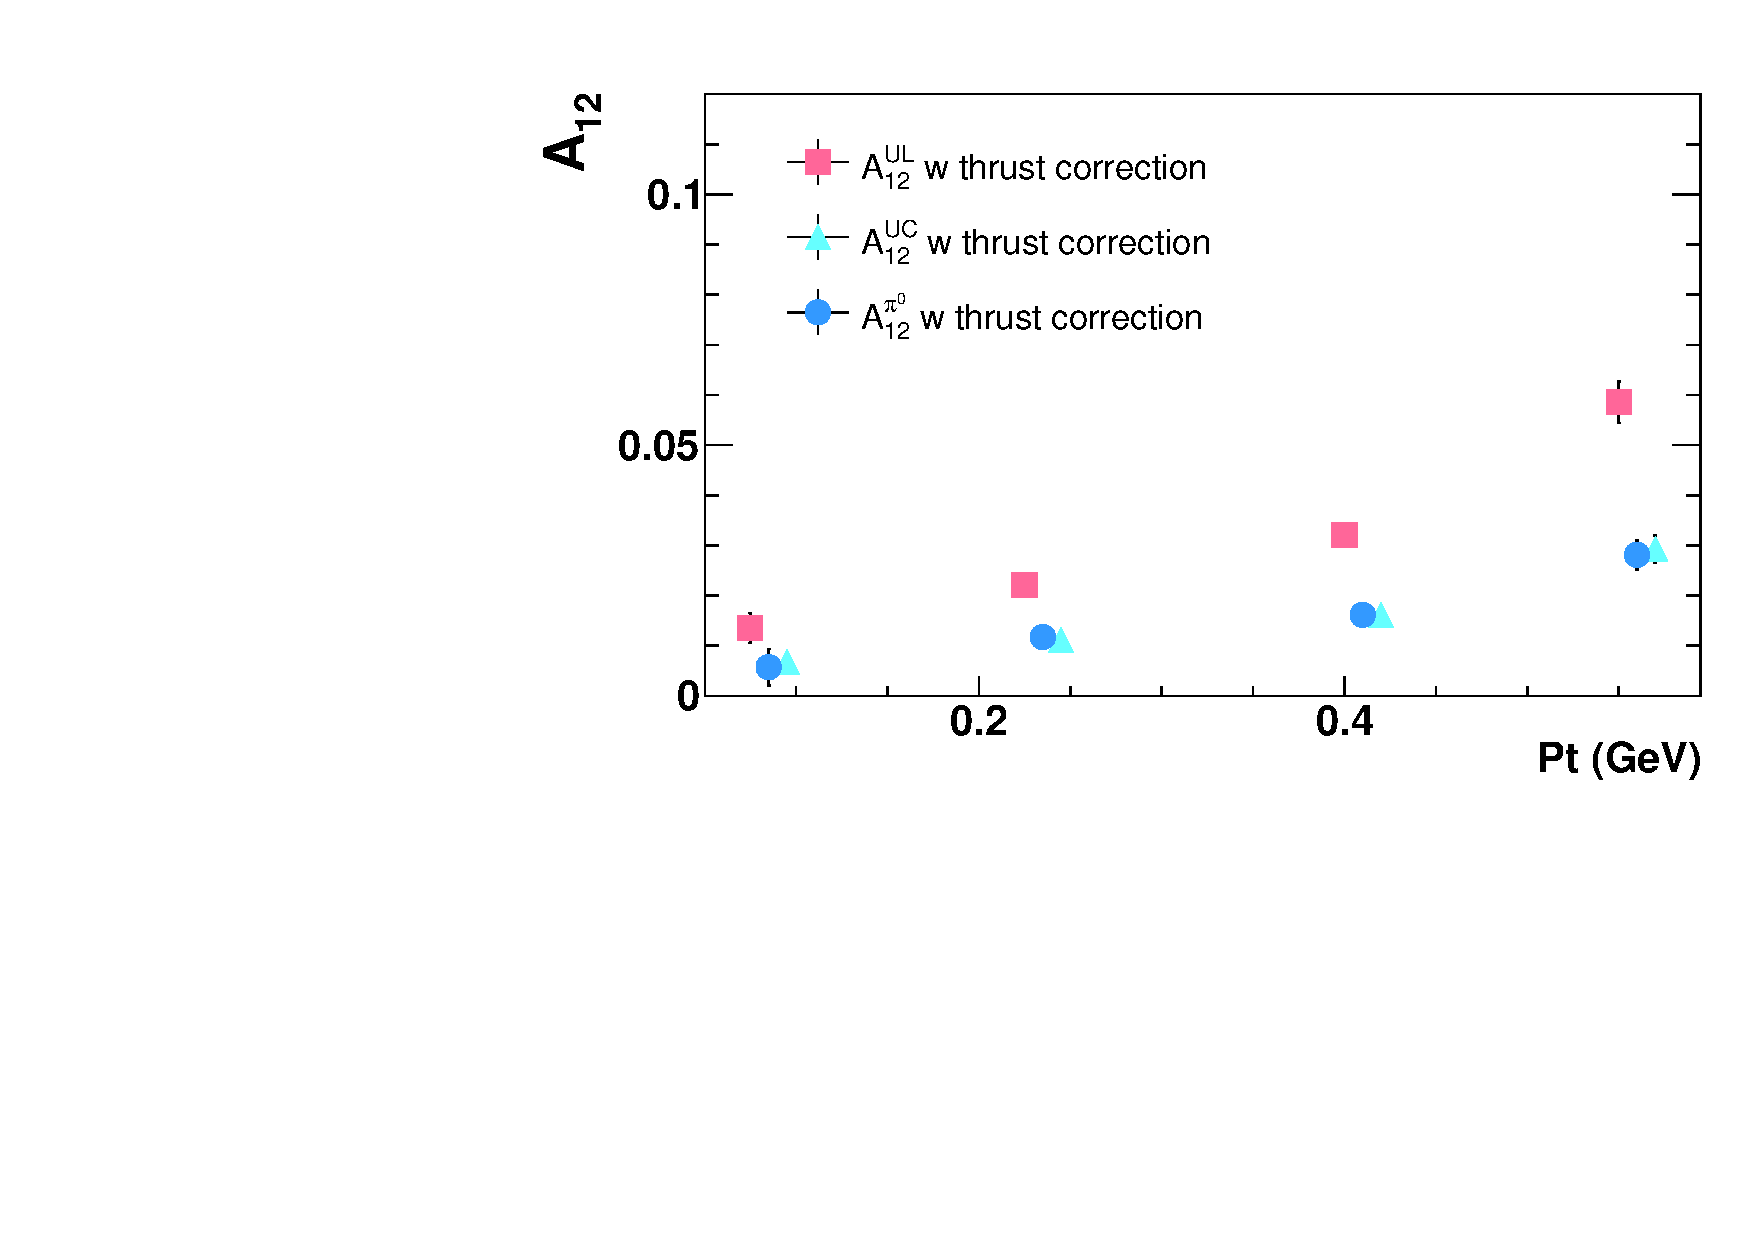
\includegraphics[width=60mm,natwidth=600,natheight=400]{figure_asy/NeutralVsCharge_w_correction2.pdf}}
  \subfigure[$(z_1,z_2)$ bins]{\label{fig:comzCN2}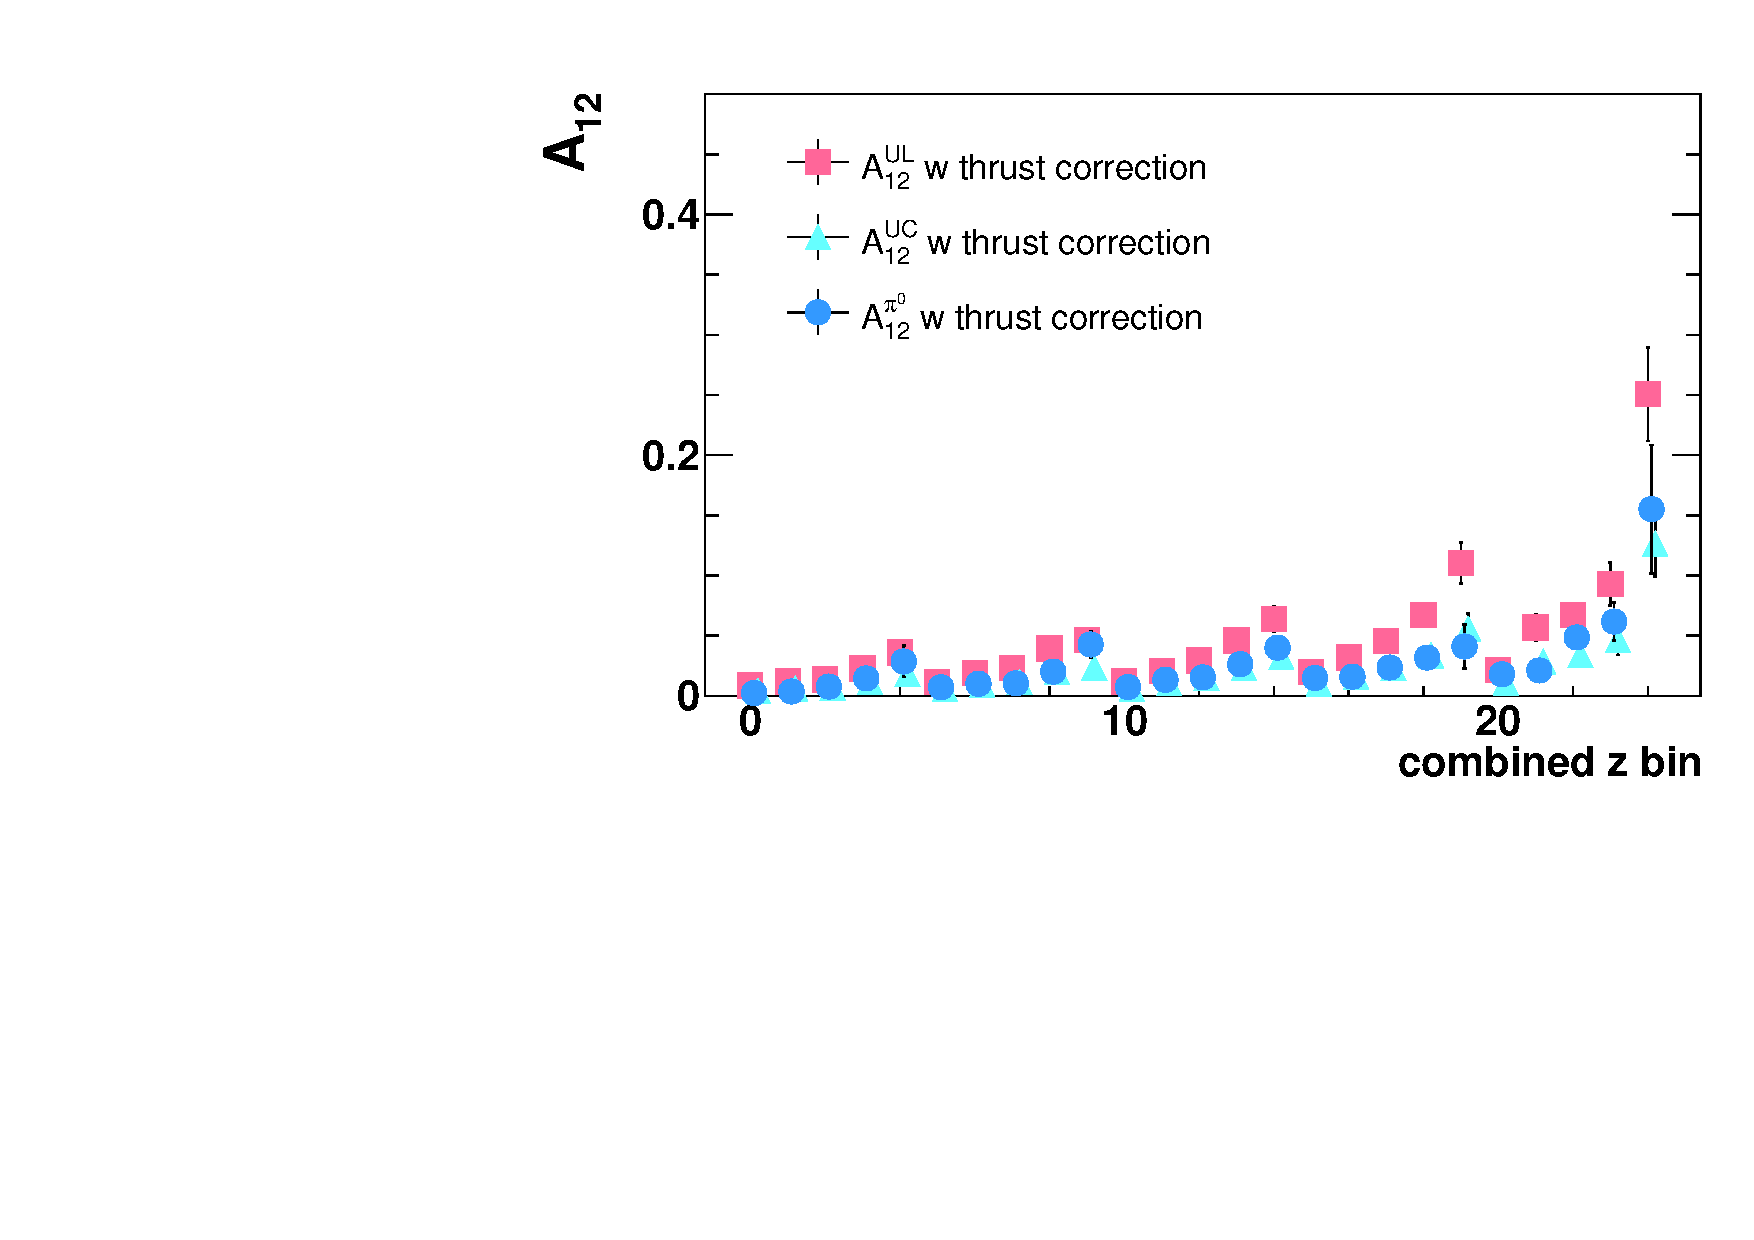
\includegraphics[width=60mm,natwidth=600,natheight=400]{figure_asy/NeutralVsCharge_w_correction1.pdf}} 
  \subfigure[$(P_{t1},P_{t2})$ bins]{\label{fig:comptCN2}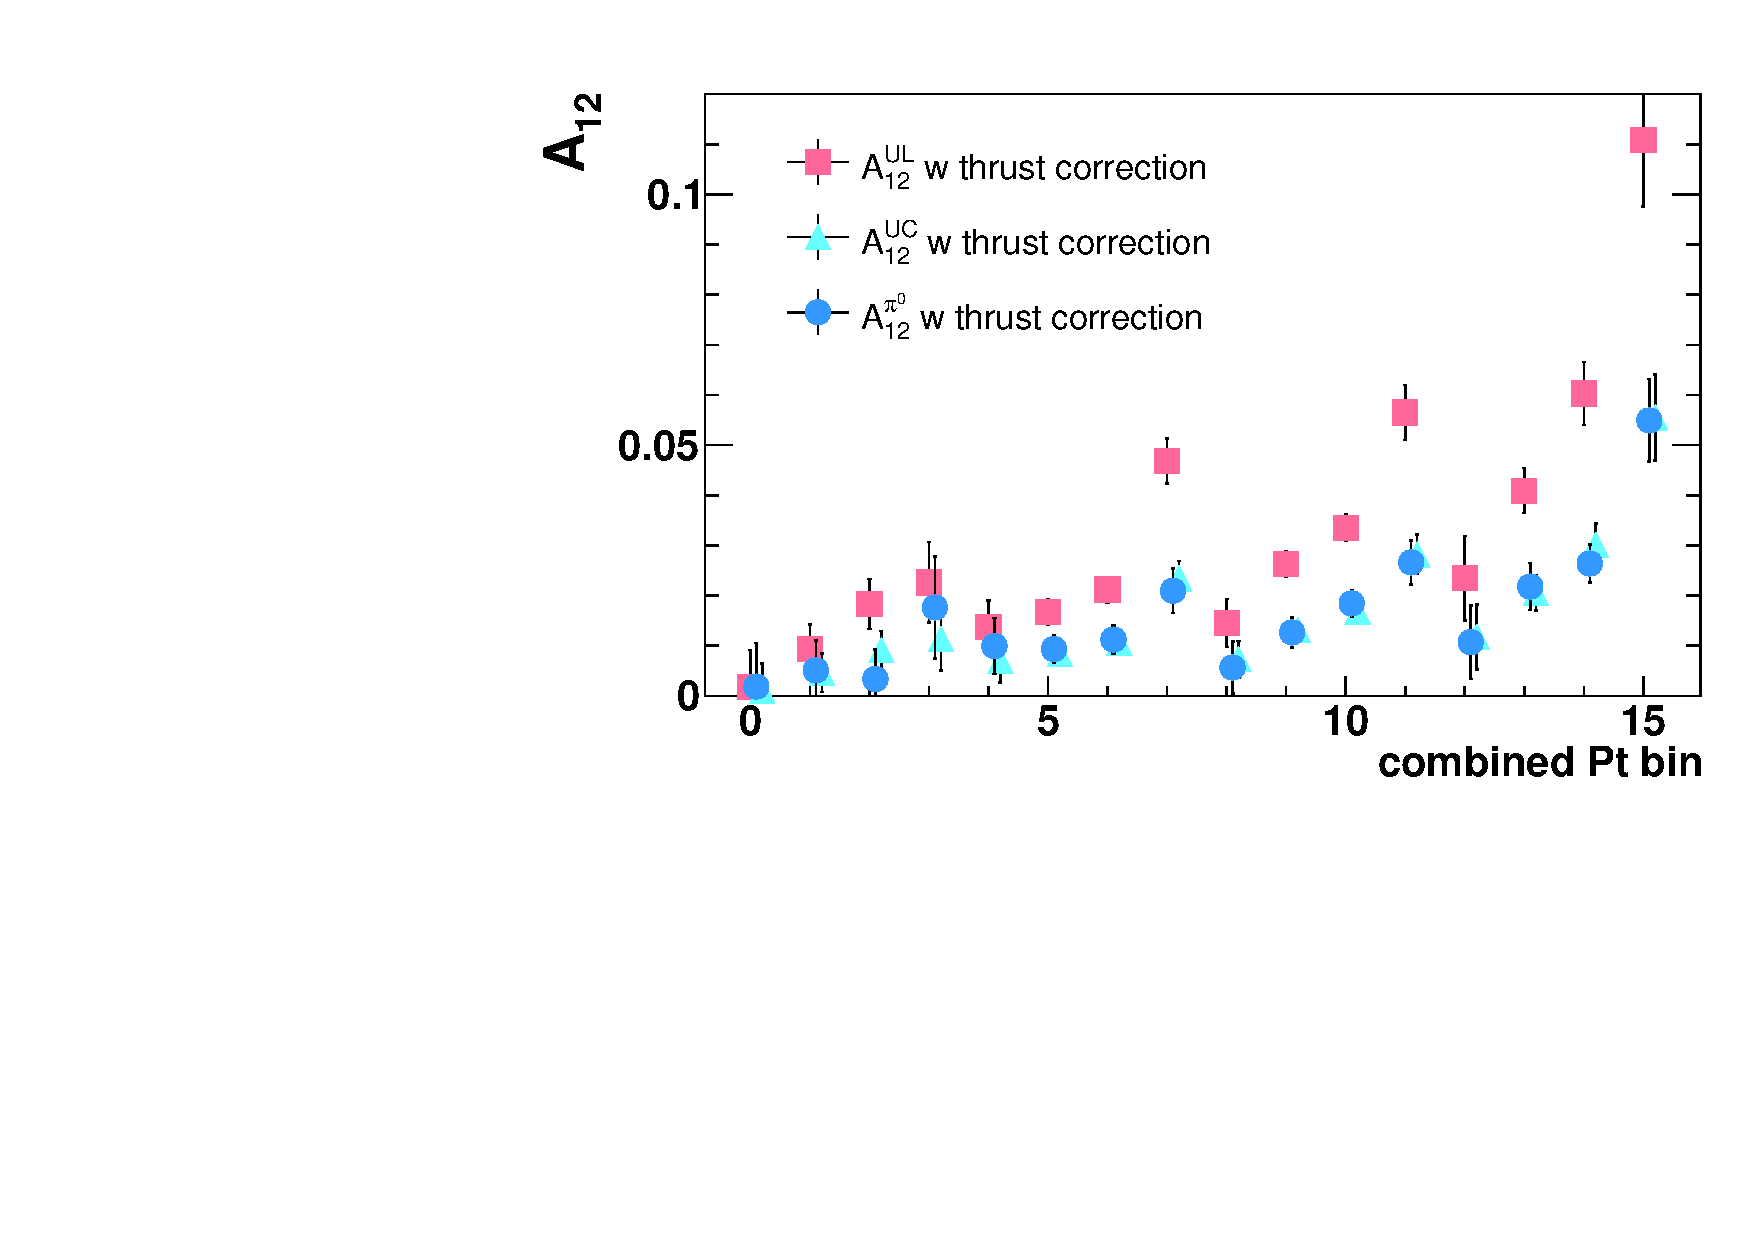
\includegraphics[width=60mm,natwidth=600,natheight=400]{figure_asy/NeutralVsCharge_w_correction3.pdf}}
  \caption{Charged pion double ratio and $\pi^0$ double ratio after thrust correction. $\pi^0$ double ratio has been modified for background correction. The square, triangle and round points are UL, UC and $\pi^0$ asymmetries, respectively.}
\label{fig:pionCNcorrection}
\end{figure}

In \cite{BabarCharged}, Collins asymmetry for charged pions is studied based data collected by BABAR experiment. However in this studies, mis-PID correction and charm contribution are not considered and the thrust smearing correction factors are applied on the corresponding bins while the other two researches use a average correction factor. Also the smearing correciton factor was calculated using real $q\bar{q}$ axis in previous studies while here we use stable thrust axis. And tighter fiducial constraint applied may increase the statistical uncertainties as well as the Collins asymmetry.% Different kinematic bins are assigned and only the bin with $0.5<z_1<0.7, 0.5<z_2<0.7$ is the same with $(z_1,z_2)$ bins 7 in this note. The comparison is listed in Table~\ref{tab:compare}. There are many possible reasons for the difference between measurement. In this note mis-PID correction and charm contribution are not considered and the thrust smearing correction factors are applied on the corresponding bins while the other two researches use a average correction factor. Also tighter fiducial constraint may increase the statistical uncertainties as well as the Collins asymmetry.

\iffalse  
\begin{table}[H]\footnotesize
\centering
\begin{tabular}{|l|l|l|l|l|l|l|l|l|l|l|l|l|l|l|l|l|l|}
\hline
$z_1$ & $z_2$ &  Babar & Belle previous &This Note \\ \hline
UL&[0.5,0.7]&[0.5,0.7]& 10.97$\pm$0.73$\pm$0.62& 11.30$\pm$0.26$\pm$0.53 & 9.97$\pm$0.68-0.13/+0.67 \\ \hline   
UC&[0.5,0.7]&[0.5,0.7]&4.56$\pm$0.6$\pm$0.37&   & 5.37$\pm$0.52-0.13/+0.37 \\ \hline
\end{tabular}
\caption{Variables and results of background correction for $\pi^0$ $z_1$ bins. All numbers are in percent.}
\label{tab:compare}
\end{table}
\fi
